\documentclass[oneside]{book}

\usepackage{graphicx}
\graphicspath{ {./images/} }
\usepackage{amsthm}
\usepackage{amsmath}
\usepackage{mathrsfs}
\theoremstyle{definition}
\newtheorem{definition}{Definition}[section]



\title{Dispensa Intro to Machine Learning}
\author{Bonmassar Ivan}

\begin{document}
	\maketitle
	\tableofcontents
	
\chapter{ML Basics}
The main notion to get from this is the following. ML allows computers to gain \textbf{knowledge} acquired through \textbf{algorithms} by learning from data. This knowledge is represented through a \textbf{model} which is then used on future data.

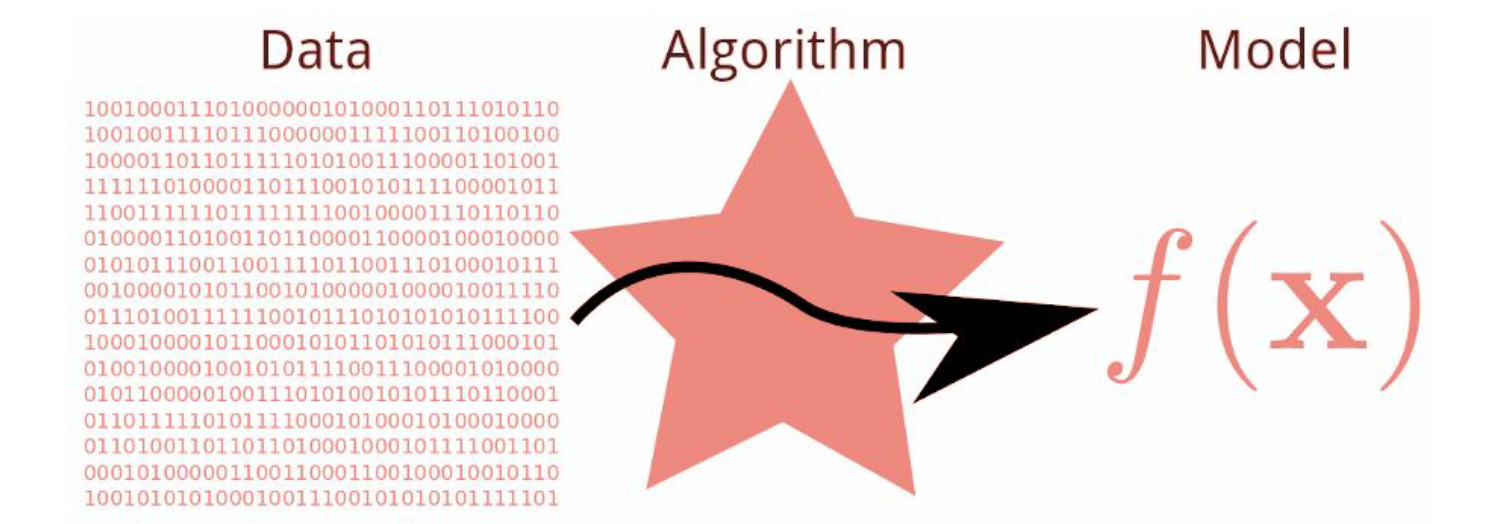
\includegraphics[scale=0.25]{data_model}

The training data produces a model or predictor, whereas the testing data produce a prediction. 
\section{Data}
Data can be a list of movies from IMDB which is easily representable. Although we need to use \textbf{features} when taking into consideration other examples. Features is how an algorithm view data and is generally represented with vectors. 

For example, classifying different apples, features could be the shape and colour of them.

The general problem with data for classification for example is that not all data is the same. For instance a banana can either be green or yellow. Although this is true we cannot go to deep with this so we use a probabilistic model called \textbf{data generating distribution}. Both training and test data are based on this. 

So in our previous example, we will generalize and say that bananas are yellow. 

\begin{definition}[Probability distribution]
	Describes how likely certain events are.
\end{definition}

High probability: round apples

Low probability: square apples

\section{Types of Learning}
\textbf{SUPERVISED LEARNING}\\
Supervised learning is when the algorithm is given labeled examples and the predictor should output a label. A further example of this is \textbf{classification}, where the model classifies from a pool of categories. 

Given a training set $T = {(x_i, y_i)}$ learn a function that predicts $y$ given $x$. x is multi-dimensional.

Some real world examples can be facial recognition, spam detection and character recognition. 

\textbf{Regression} is similar to classification only with real values (i.e. numbers).

\textbf{Ranking} the label is a ranking (most similar, most popular web pages etc.)


\textbf{UNSUPERVISED LEARNING}
The given data is without labels. 
Some examples are: 

\textbf{Clustering}, where the output is the general structure of the data set (clusters of data). Real world examples are image segmentation, social network analysis 

\textbf{Anomaly detection}

\textbf{Dimensionality reduction} 

\textbf{REINFORCEMENT LEARNING}

The idea is that the agent interacts with the environment and receives rewards based on behavior. 

\section{ML Ingredients}

\textbf{TASK}

A task represents the type of prediction being made to solve a problem. 

Assigning each input $ x \in \mathscr{X}$ to an output $y \in \mathscr{Y}$

\textbf{Data}

Data is basically the information required to solve a specific problem and as said previously is usually sampled from an unknown data generating distribution :

$\textbf{p}_{data}$ 

For classification and regression $\textbf{p}_{data} \in \triangle (\mathscr{X} \times \mathscr{Y})$

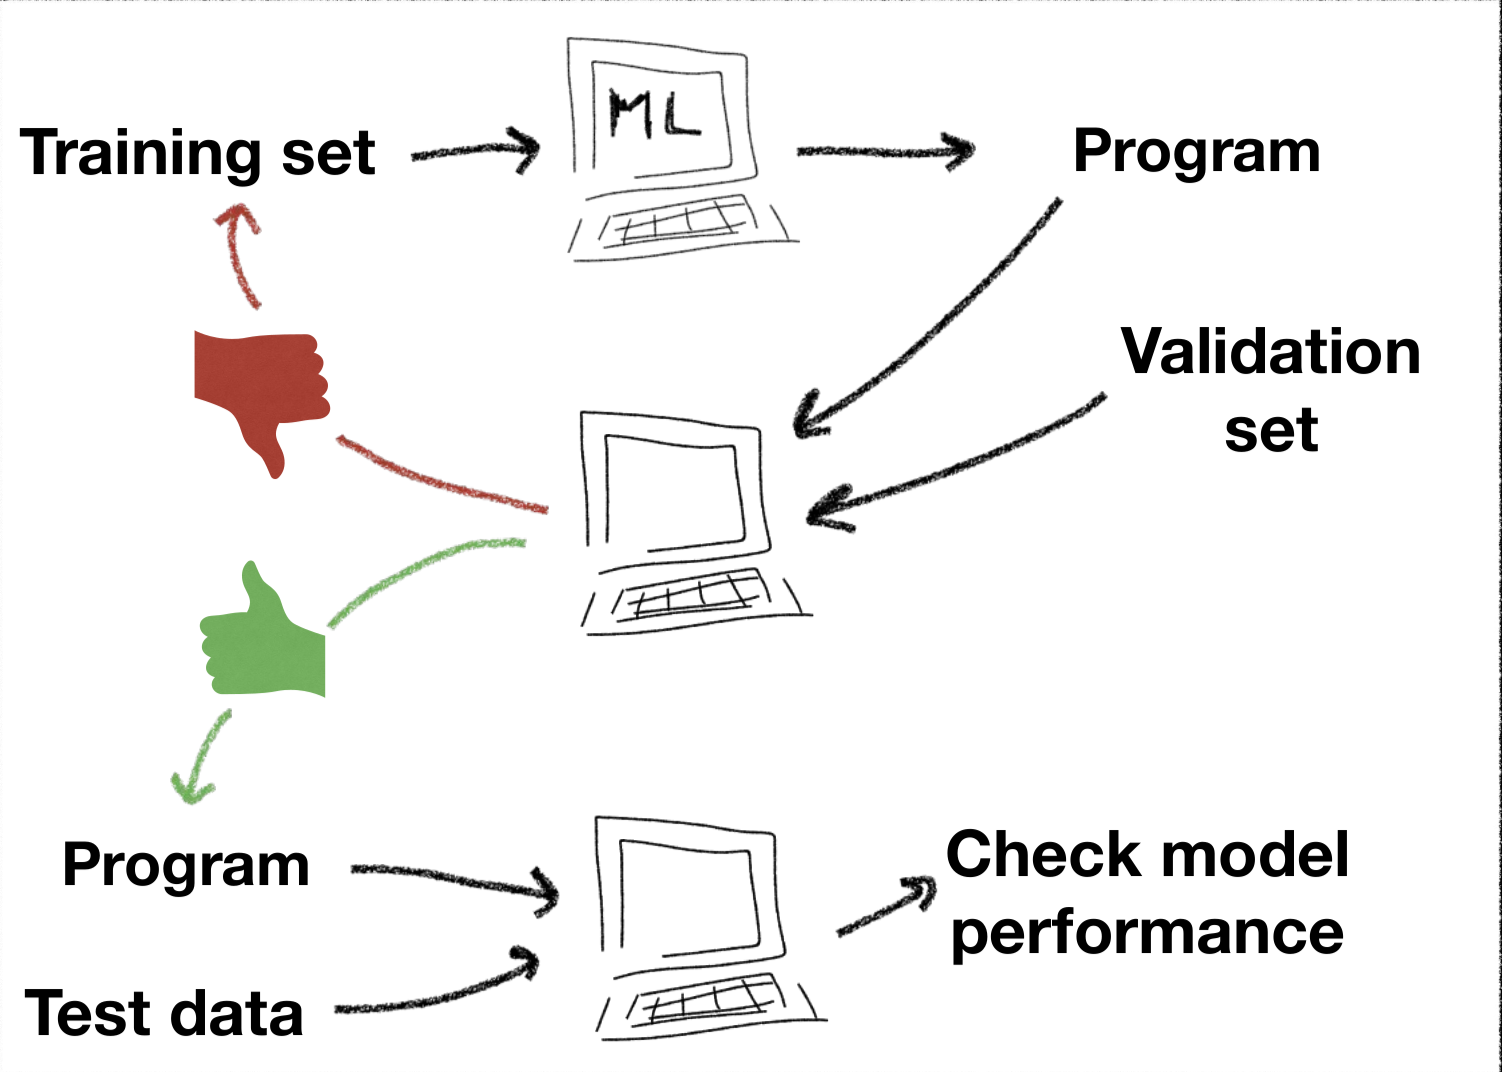
\includegraphics[scale=0.25]{datasets}

\textbf{Model and hypothesis space}

A model is like a program that solves the problem. There are various models (decision trees, neural networks.. ) and a set of them makes up the hypothesis space. 

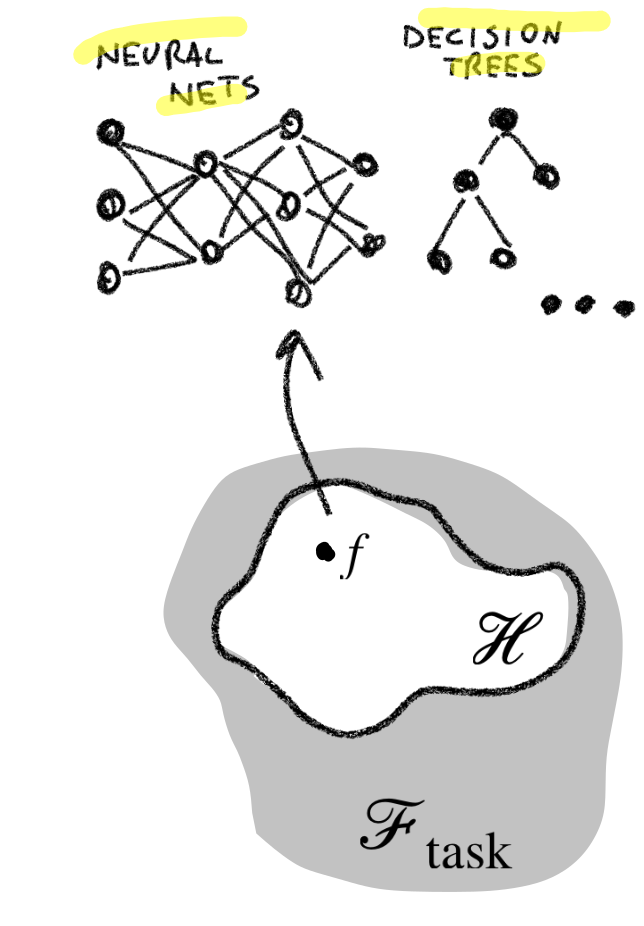
\includegraphics[scale=0.24]{hypothesis_space}

\textbf{The objective}

The objective is to minimize an error function $E(f,\textbf{p}_{data})$ to find the optimal function 

$f^{\star} =$ arg min $E(f,\textbf{p}_{data}) $.

This however is really hard to do because of the too large search space. 

The \emph{feasible target} is the optimal one in a restricted hypothesis space $\mathscr{H}$

$f^{\star}_{\mathscr{H}} =$ arg min $E(f,\textbf{p}_{data}) $.

This is also not doable because we do not have access to $\textbf{p}_{data}$
\\
The \emph{actual target} is then the following: 
\\

$f^{\star}_{\mathscr{H}} (\mathscr{D}_n) =$ arg min $E(f, \mathscr{D}_n) $. where $\mathscr{D}_n$ is a training set. 

The error function is usually specified as a pointwise-loss $\mathscr{l}(f,z)$ measuring the error of f on the training set z. 

The learning algorithm solves the optimization problem which targets the actual target. 


\chapter{K-Nearest Neighbor}

Imagine assigning each feature a numeric value, and putting them as coordinates in a feature space. To find which label to give to an example $d$ we can see the k-nearest neighbors. The correct label will be the one that has the majority in k neighbors. 


In cases where features are comparable (each feature has the same units) we will use the simple method of Euclidean Distance: 

\[
D(a,b) = \sqrt{(a_1-b_1)^2+(a_n-b_n)^2}
\]

\section{Decision boundaries}

\begin{definition}[Decision boundaries]
	Decision boundaries are places where the the classification of an example changes.
\end{definition}

These boundaries are a subset of the Voronoi diagram which divides the initial points distribution by equidistant lines. 

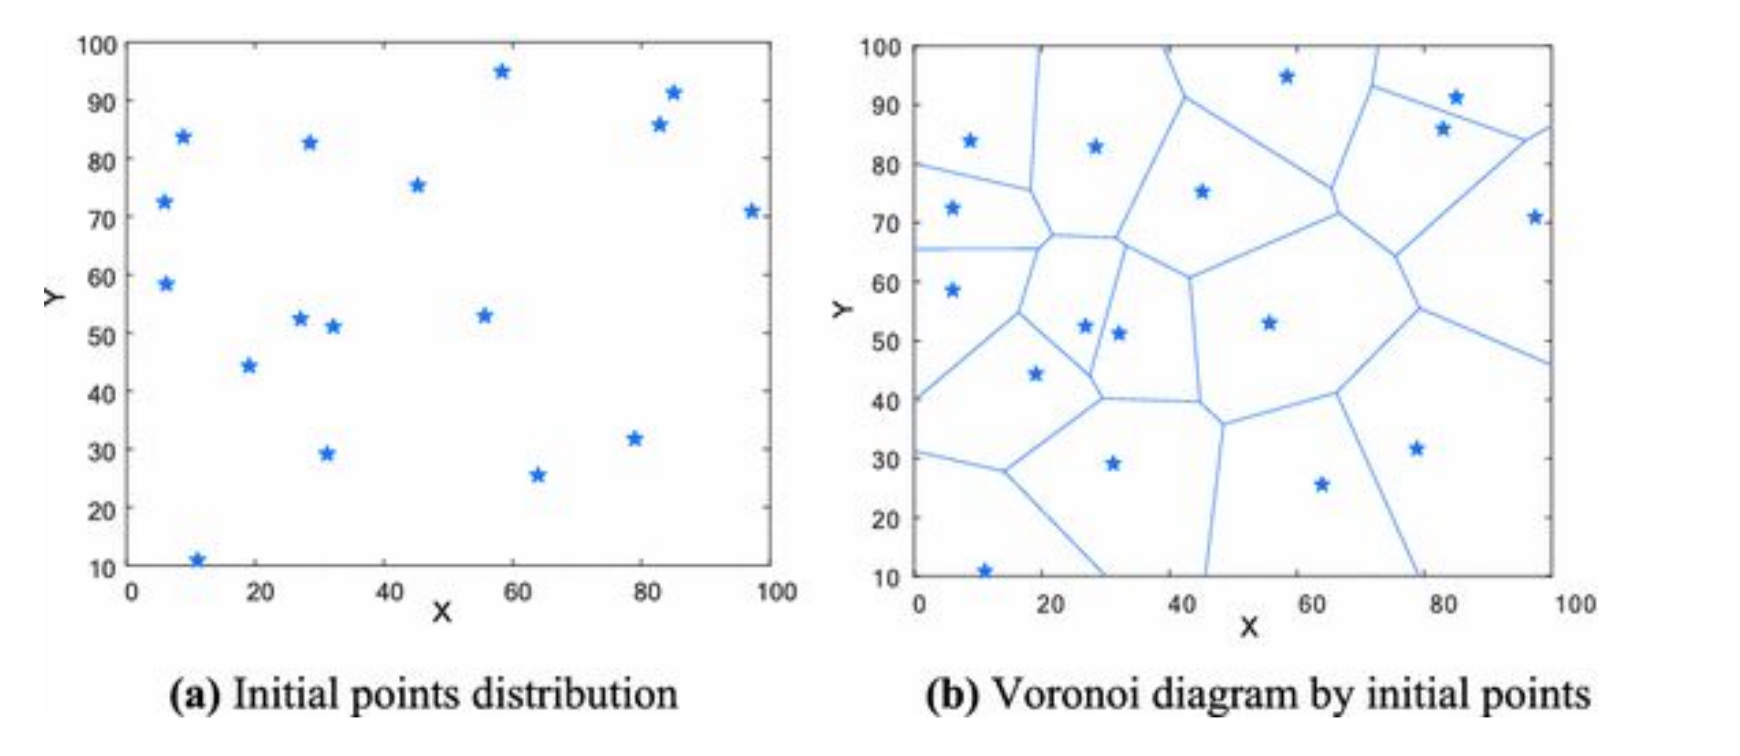
\includegraphics[scale=0.2]{voronoi}

Choosing K will have an effect on underfitting and overfitting.

\begin{definition}[Underfitting]
	Underfitting occurs when the model is not able to achieve a low error value on the training set
\end{definition}

\begin{definition}[Overfitting]
	Overfitting occurs when the gap between training set error and test set error is large
\end{definition}

Some heuristics come into play. It's important to choose an odd number to avoid ties. A general rule of thumb is that k should be lower than the square root of N training examples.
\\
\textbf{Weighted k-nn}, uses the same mechanics only that the examples are weighted which means that they will weigh in more in a vote situation.

\textbf{Lazy learning} is when an algorithm simply stores data and operates when given a test example.

\textbf{Eager learning} on the other hand is when given a training set, the algorithm constructs a classification model which then reutilizes. 

\section{Summary}
When is it useful:
\begin{itemize}
	\item Few features per instance
	\item Lots of training data
\end{itemize}

Advantages:

\begin{itemize}
	\item Training is very fast (lazy)
	\item Learn complex functions
\end{itemize}

Disadvantages:

\begin{itemize}
	\item Slow at query time
\end{itemize}





The main issue has to do with dimensionality. Every algorithm requires a dense data set, although K-NN requires to have at least one neighbor in each dimension, which makes for a very heavy computational load.

\chapter{Linear Models}
\section{Model assumptions}
Assumptions (when correct) are a great tool to improve an algorithm. They can however lead to overfitting. For K-NN the only assumption that's made is the fact that proximity relates to label. 

\begin{definition}[Bias]
	The bias of a model is how strong its assumptions are.
\end{definition}

K-NN and Decision Trees are considered to be low bias. 

\section{Linear models}
A high-bias assumption is linear separability, which means that the classes can be simply divided by a line (or hyperplane in n dimensions).

A line is defined by a pair of values: 

\[
0 = w_1f_1 + w_2f_2
\]

To classify we can input the values into the equation. If it's positive it will be above the line and viceversa.

In n-dimensions: 

\[
0 = b+ \sum_{i=1}^{n} w_if_i
\]

\section{Online learning}

This linear model is different because it sees one example at a time. This is useful when taking in data streams (for example from online resources).

The algorithm receives an unlabeled example, it predicts and if it is not correct it updates its model.

\section{Perceptron algorithm}
This is a linear model that constantly updates when not correct.

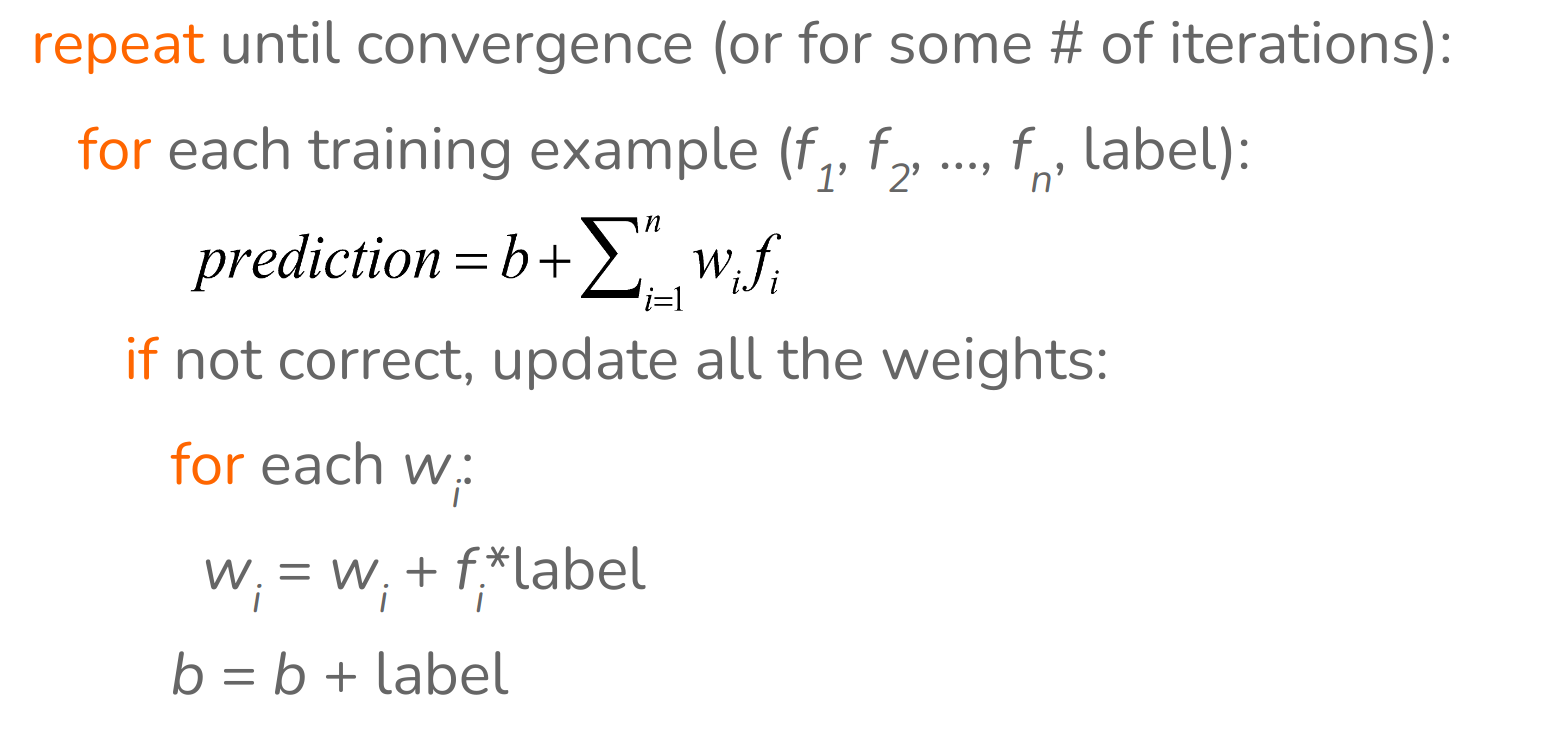
\includegraphics[scale=0.25]{perceptron}

\chapter{Multiclass Classification}
\begin{definition}[Binary classification]
	Given an input $\mathscr{X}$, an unknown distribution $D$ over $\mathscr{X}\times \{-1,1\}$
	a training set D compute a function f.
\end{definition}

\begin{definition}[Multiclass classification]
	Given an input $\mathscr{X}$ and a number K of classes, an unknown distribution $D$ over $\mathscr{X}\times K$
	a training set D compute a function f.
\end{definition}

None of the current methods work.

The main idea is to modify the perceptron by adding multiple lines. There are two approaches to this.

\section{One vs All (OVA)}

For each label L define a binary problem. All examples with L are positive, the rest is negative.

This poses a problem related to some areas in which it can either be two classes or none at all.

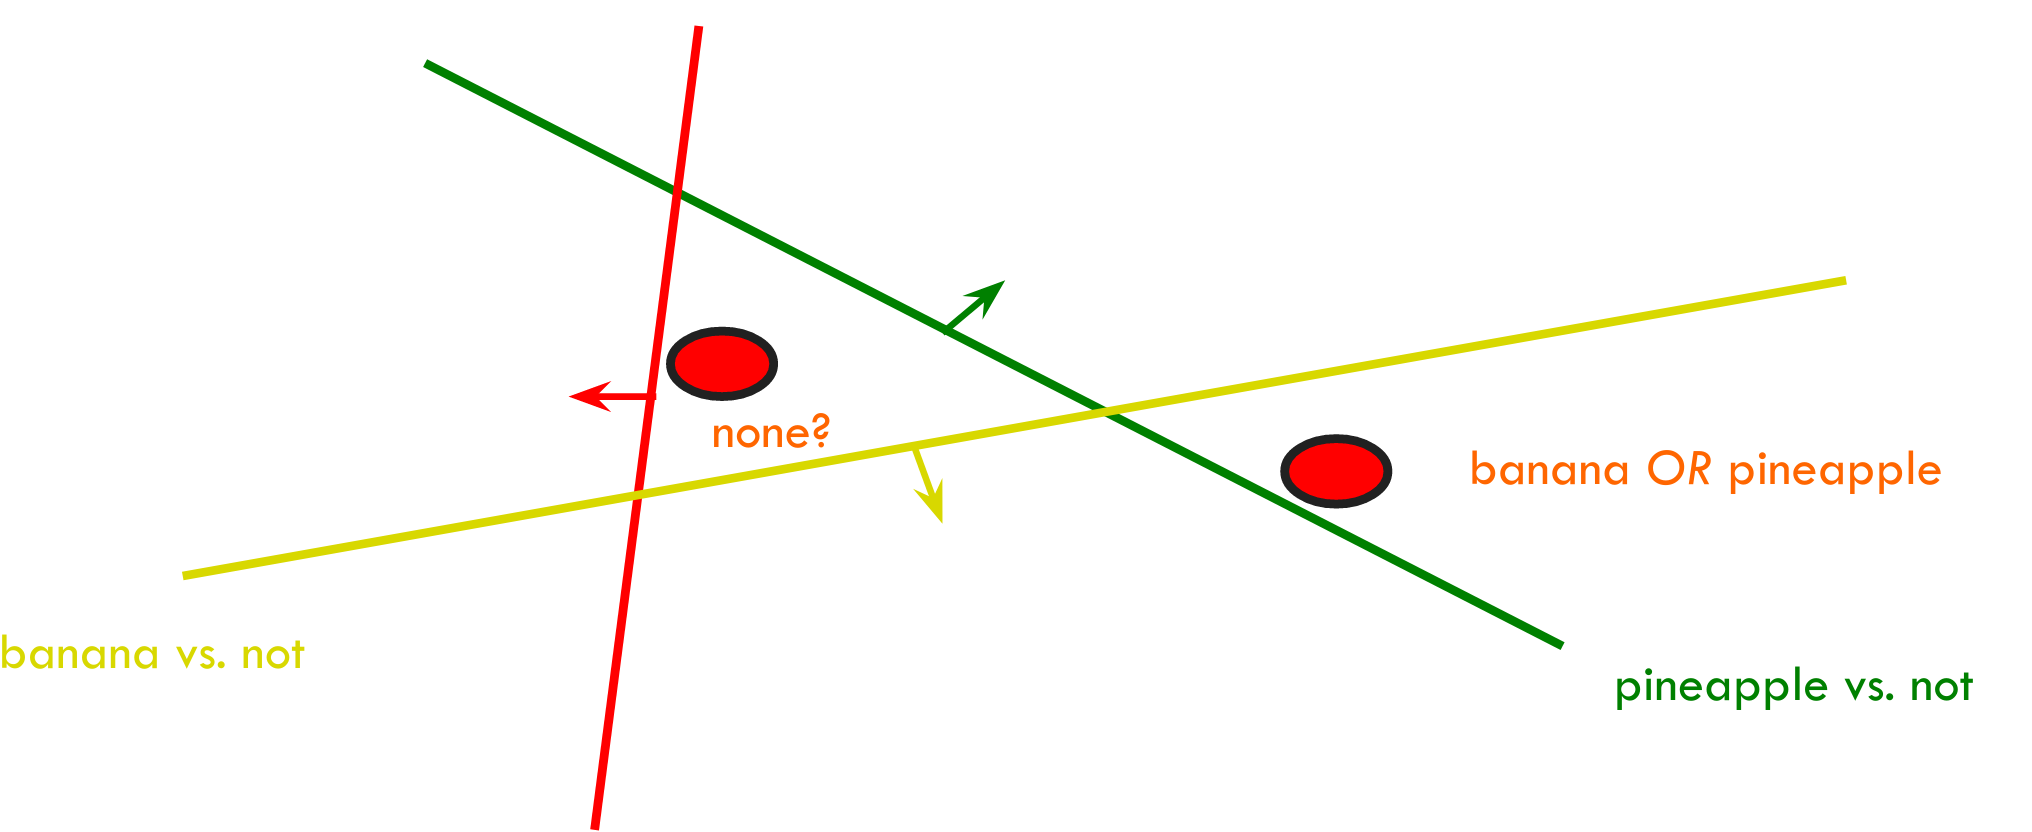
\includegraphics[scale=0.1]{multiclass}
 How to classify? 

Generally speaking the classifier should provide a level of confidence. To calculate this value we need to use decision boundaries and its distance from the hyperplane.
 
\section{All vs All (AVA)}
The idea behind AVA is to pair up each permutation of 1v1 pairs. Then, the classifier will receives all examples of i as a +1 and -1 for the j class. When a test point arrives we evaluate on all the $F_{ij}$ classifiers. 

\section{Summary}
AVA has faster training time but a slower test time. AVA has more chances of error at test time.

\textbf{Evaluation} comes when we need to evaluate a specific performance of an algorithm. Can be done through microaveraging, average over the examples, or macroaveraging, average of the average of each label.



\chapter{Gradient Descent}
\section{Model based machine learning}
There are 3 steps to this model:
\begin{enumerate}
	\item Pick a model (DT, perceptron)
	\item Pick a criterion to optimize
	\item Develop a learning algorithm
\end{enumerate}

In linear model: 
\begin{enumerate}
	\item 0 = b+ $\sum_{j=1}^{n} w_jf_j$
	\item $\sum_{i=1}^{n}1[y_y(w\cdot x_i + b) \leq 0]$ (0/1 Loss function aka the total number of mistakes)
	\item $argmin_{w,b}$ $\sum_{i=1}^{n}1[y_y(w\cdot x_i + b) \leq 0]$
\end{enumerate}

\section{Surrogate loss functions}
Minimizing the 0/1 Loss function is an NP-hard problem, because of the many local minima and any change in w can change drastically the result. Ideally we would want a convex function so to have at least one minimum.

By \textbf{surrogate loss function} we mean a loss function that provides an upper bound to the 0/1 loss function. 

\begin{itemize}
	\item 0/1 loss : $l(y,y') = 1[yy'\leq 0]$
	\item Hinge loss: $l(y,y') = max(0,1-yy')$
	\item Exponential loss: $l(y,y') = exp(yy')$
	\item Squared loss: $l(y,y') = (y-y')^2$
\end{itemize}

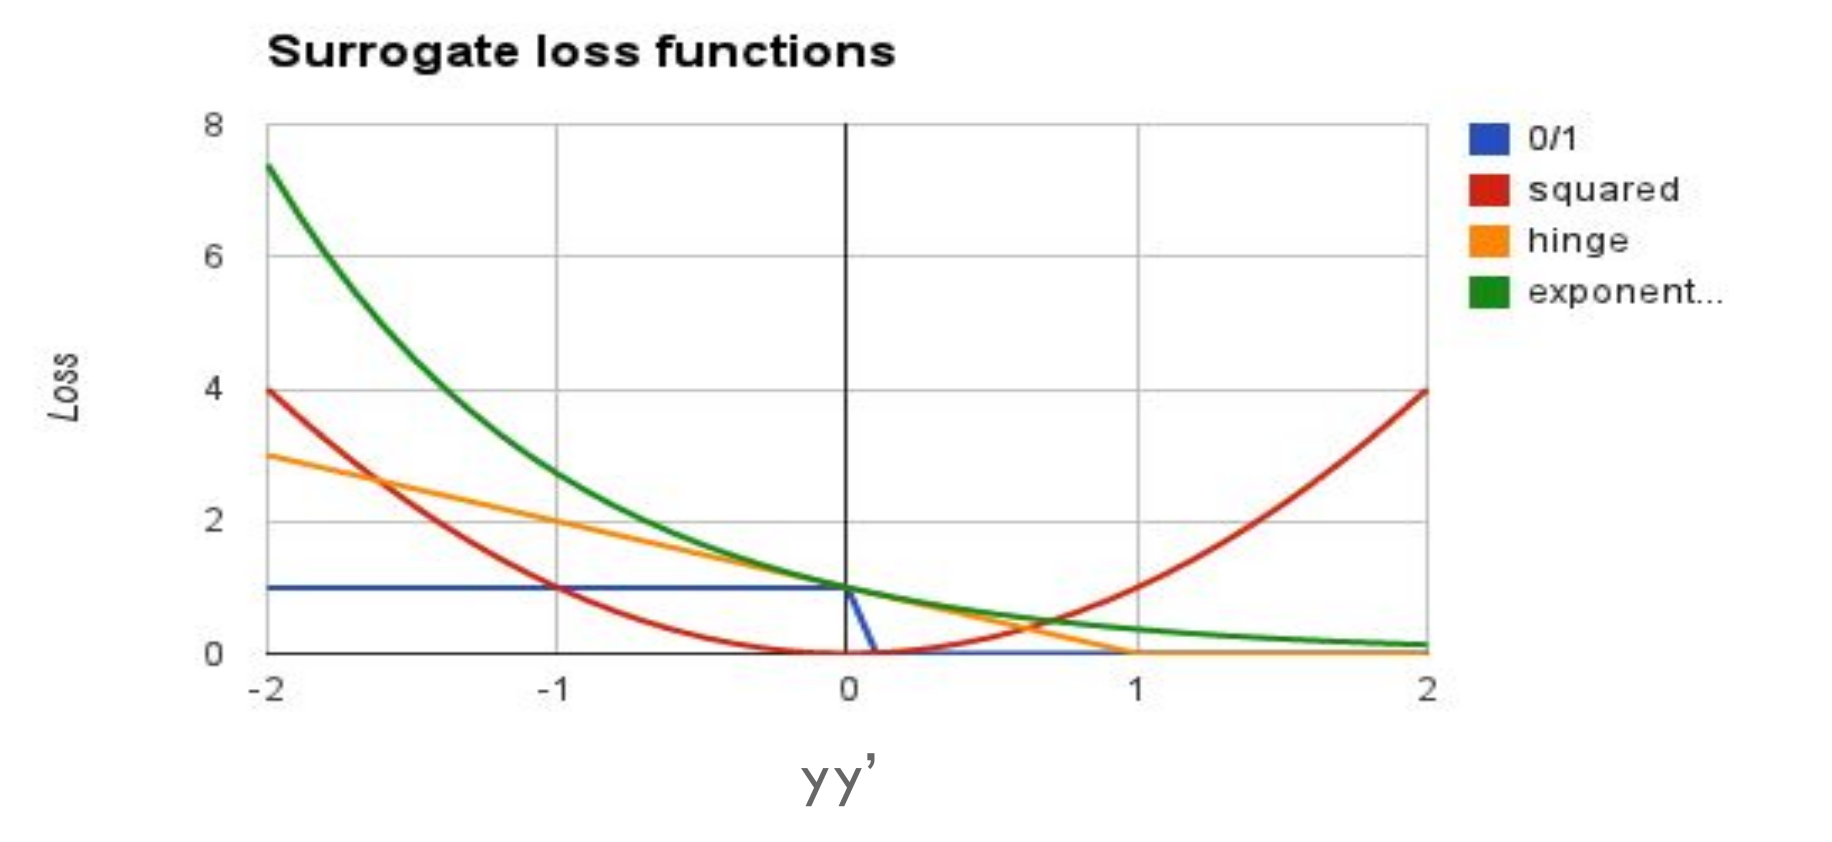
\includegraphics[scale=0.2]{surrogate}

\section{Gradient descent}
We use gradient descent to find a minimum in the function. 

The general approach is to choose a starting point $w$, calculate the derivative and move in that direction.

\[
w_j = w_j - \eta \frac{d}{dw_i}loss(w)
\]



$\eta$ is the rate at which we move and will change over time.

Since it's changing over time it can be implemented through a perceptron algorithm.

The main problem with gradient descent is local minima: 

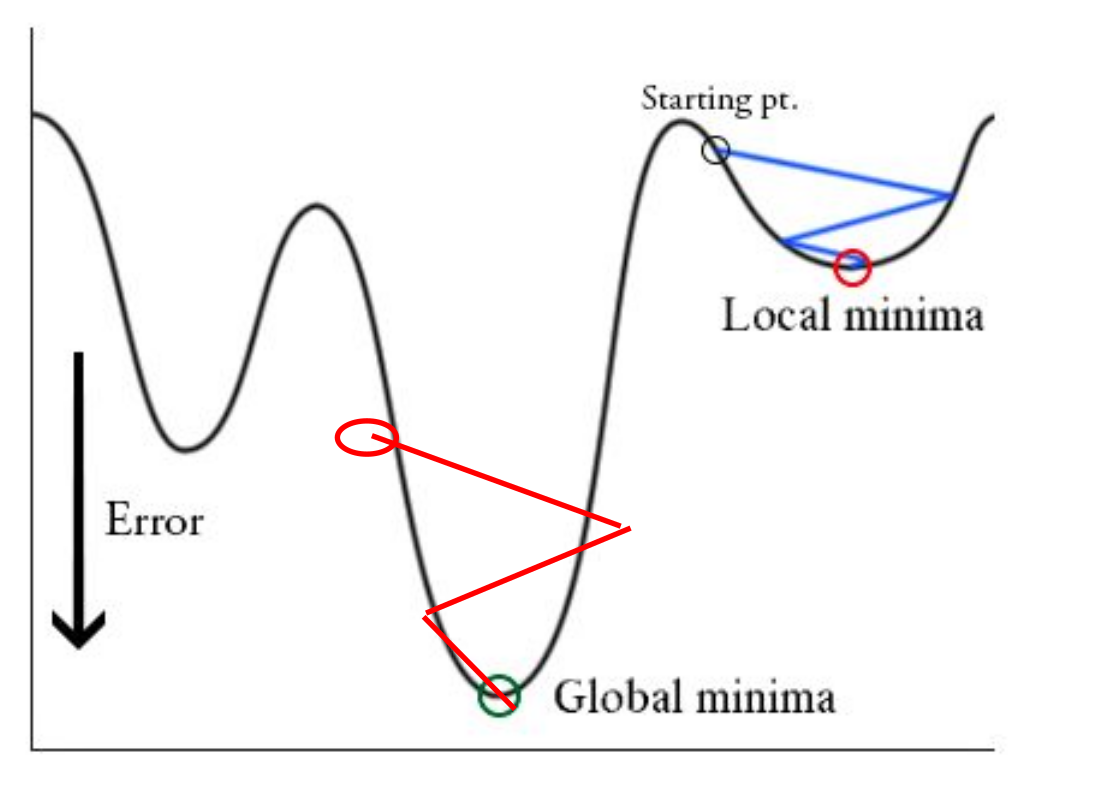
\includegraphics[scale=0.2]{local_minima}

\chapter{Regularization}
The problem with gradient descent remains the fact that since we're using it on the training set it can lead to overfitting. A solution to this is to use a regulalrizer.

\begin{definition}[Regularizer]
	An additional criterion to the loss function to avoid overfitting.
\end{definition}

More generally it regularizes the way we handle certain weights.

Generally, we do not want huge weights: if weights are large, a small change in a feature can result in a large change in the prediction.

Two common regularizers are: 

\begin{itemize}
	\item Sum of the weights: $\sum |w_j|$
	\item Sum of the squared weights: $\sqrt{\sum |w_j|^2}$
\end{itemize}

Sum of weights penalizes small values whereas square sum penalizes large values. 

P-norm: $\sqrt[p]{\sum |w_j|^p}$

\chapter{Support Vector Machines}

In linear classifiers there are two variations: 
\begin{itemize}
	\item which hyperplane to choose
	\item how does it handle non separable data
\end{itemize}

\section{Large margin classifiers}
\begin{definition}[Margin]
	The margin is the distance from the classifier to the \textbf{closest} point of either class.
\end{definition}

These points are called \textbf{support vectors} and for $n$ dimensions there are $n+1$.\\
Maximizing the margin is usually good because it means that we can only consider SVs. \\
To calculate the margin: \\
\[
\frac{w\cdot x_i + b}{||w||} = \frac{1}{||w||}
\]

To maximize the margin we need to setup a constrained optimization problem: \\
\[
max_{w,b} (\frac{1}{||w||})
\]
\\
subject to: $y_i (w\cdot x_i + b \geq 1) \forall i$\\

We can also see it as the min of $||w||$

A \textbf{support vector machine problem} is maximize or minimize a quadratic function subject to a set of linear constraints. 

\section{Soft margin}

The problem arises when the data is not linearly separable. \\
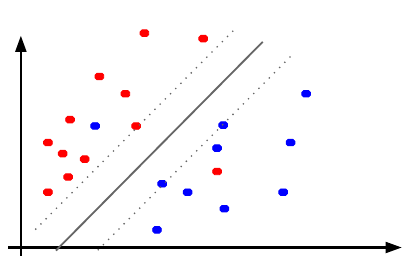
\includegraphics[scale=0.5]{non_separable}

In this case we use \textbf{slack variables} which allow for some margin of error. 
\[
min_{w,b} ||w||^2 + C \sum_{i} {\varsigma}_i
\]\\
subject to: $y_i (w\cdot x_i + b \geq 1- {\varsigma}_i) \forall i$\\

$C$ is a regularization parameter to keep overfitting under control.\\
Slack values can also be calculated: 

\begin{equation}
Slack values:
	\begin{cases}
	0 &  y_i (w\cdot x_i + b) \geq 1 \\
			1- y_i (w\cdot x_i + b) & otherwise
	\end{cases}
\end{equation}

From this we can derive an unconstrained problem: 
\[
min_{w,b} ||w||^2 +C\sum_{i}(max(0,1-y_i (w\cdot x_i + b))
\]

which is similar to a loss function with a regularizer.

An application of SVMs is for example pedestrian detection. 

\chapter{Ranking}

\section{Multiclass vs Multilabel}
Remember: multiclass classification is assigning a discrete label to a number of examples. 

For multiclass, each example has one and exactly one label, whereas with multilabel each example has 
{\bf zero} or multiple labels. \\
Some applications are: 
\begin{itemize}
	\item Reidentification
	\item Medical diagnosis
	\item Image annotation
\end{itemize}

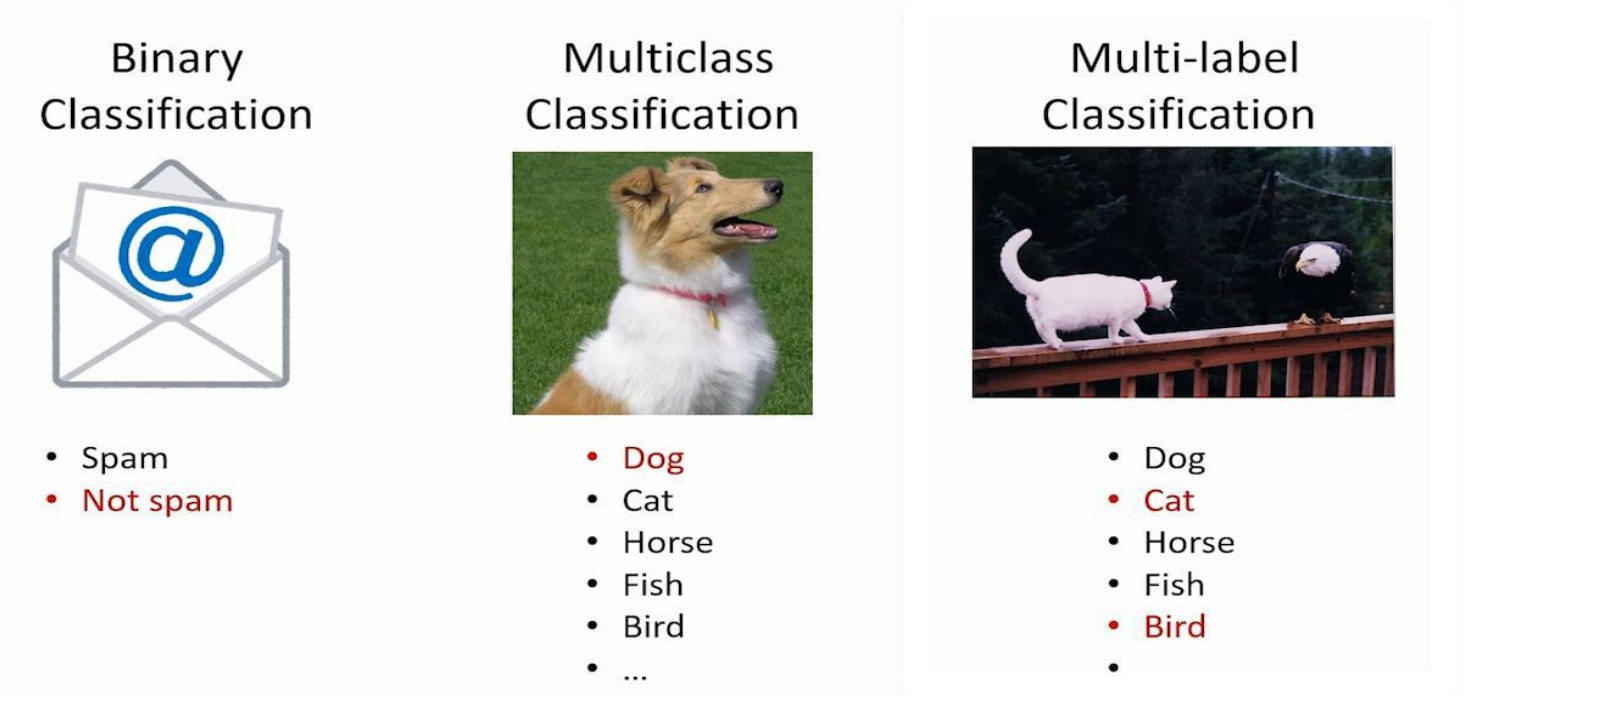
\includegraphics[scale=0.2]{classes}
\newpage
\section{Ranking}
In general the training data consists of a set of ranked examples. The {\bf ranker} will have to rank and order the test data. \\
Applications:
\begin{itemize}
	\item google search
	\item favourite movies
	\item loop closing in robotics
\end{itemize}

An approach could be using a binary classifier on pairings of examples and predict the better and worse between the two. The problem with this is that binary classifiers only take one example at the time.\\
The solution to this is to turn any pairings into one, comparing their features: 
\begin{equation}
	\begin{cases}
	1 & a_i \geq b_i \\
	0 & otherwise
	\end{cases}
\end{equation}
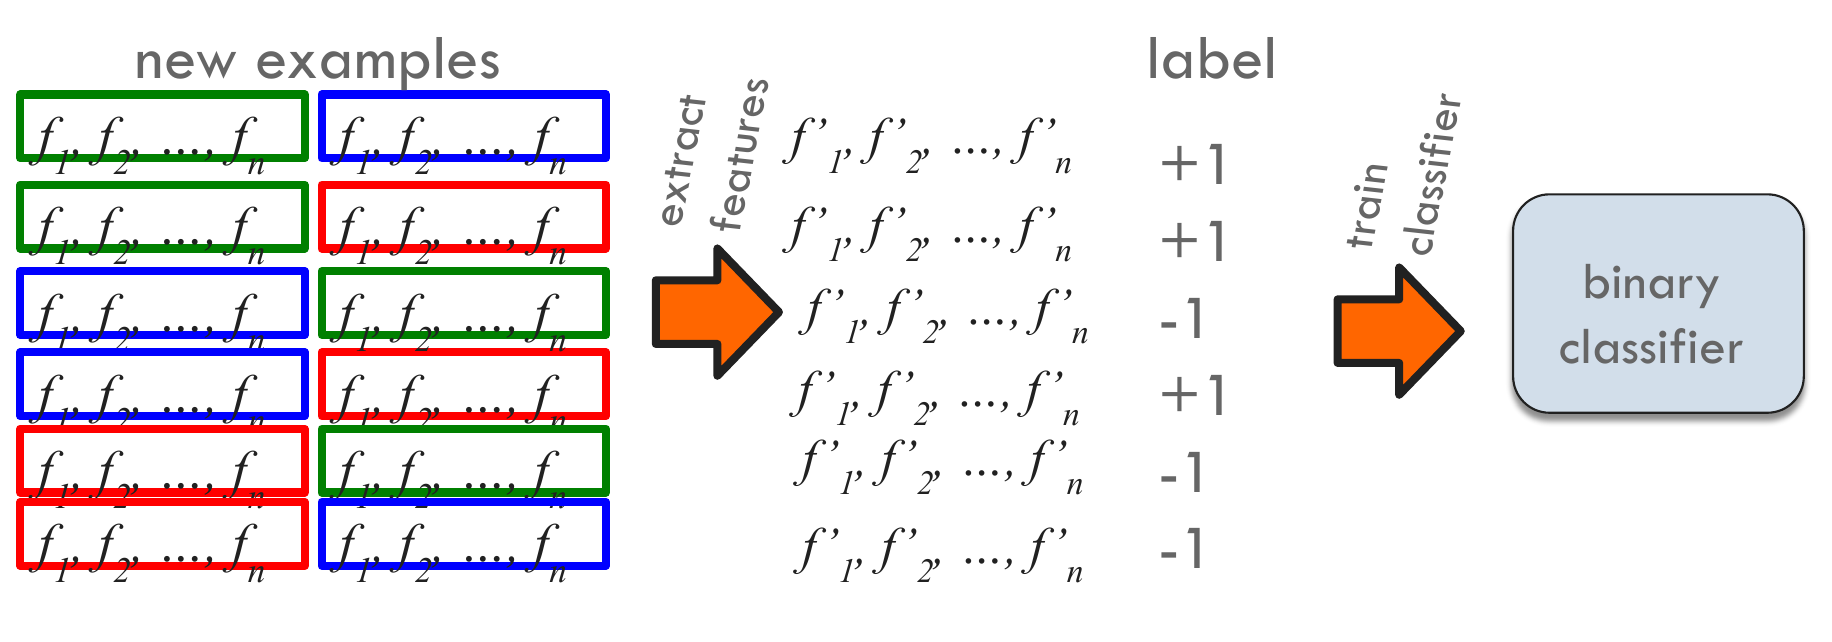
\includegraphics[scale=0.2]{ranking}

The final part of this algorithm is how to actually rank them and that's pretty straightforward: the ranking score will be equal to the sum of the rankings in the pairings. 

An application of this is if a document is relevant or not and in this case we would use a bipartite ranking system which is more similar to binary classification: is this document relevant or not? 

\chapter{Decision trees}
In decision trees each internal node corresponds to a feature, the branches correspond to a value of said feature and the leaves perform a prediction. 

It is composed of non-terminal nodes that have 2+ children and implement a {\bf routing function} and of leaf nodes which implement a prediction function.\\
A decision tree takes an input $x \in \mathscr{X}$ and routes it through the nodes until finding the final leaf, in which the prediction will take place.
\\
\\
Each non-terminal node is structured like so: \\
Node($\phi, T_L, T_R$), with a routing function $phi$ and the left and right trees underneath.
\\
On the other hand leaf nodes are Leaf(h), with h being a prediction function.
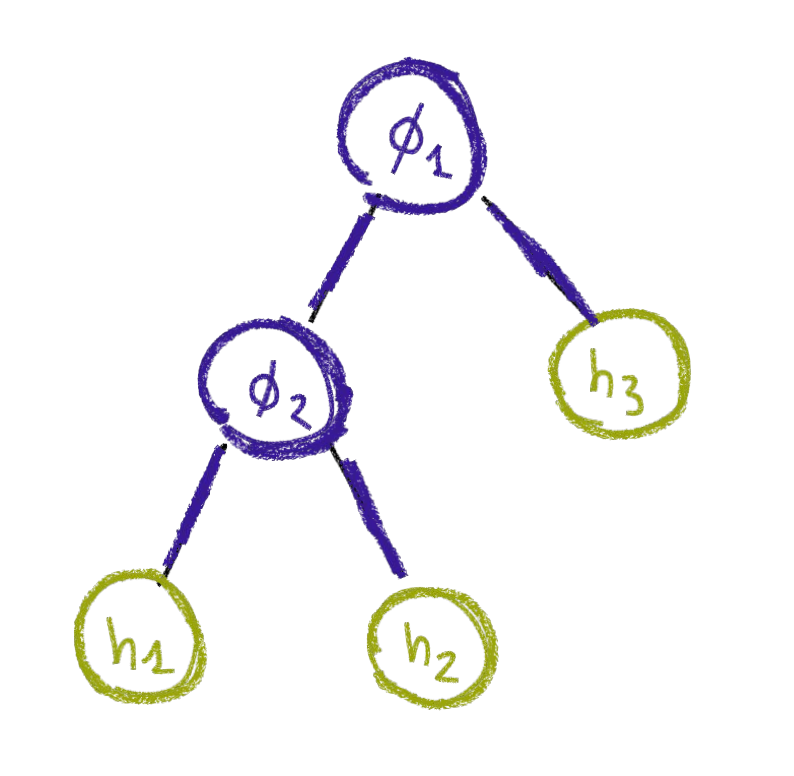
\includegraphics[scale=0.2]{dt}

\section{Growing the tree}
The main problem with growing the tree is whether we need to grow a node or a leaf. 

If a training set $\mathscr{D}$ is impure we will need to grow a node. On the other hand we will build a leaf if:

\[
I(\mathscr{D}) = E(h_{\mathscr{D}}^{\star}, \mathscr{D})
\]

As said previously if this stopping criterion is not met a node will be built with a routing function: 

\[
\phi_{\mathscr{D}}^\star \in argmin I_\phi (\mathscr{D})
\]

The impurity is computed in terms of the impurity of the split data.

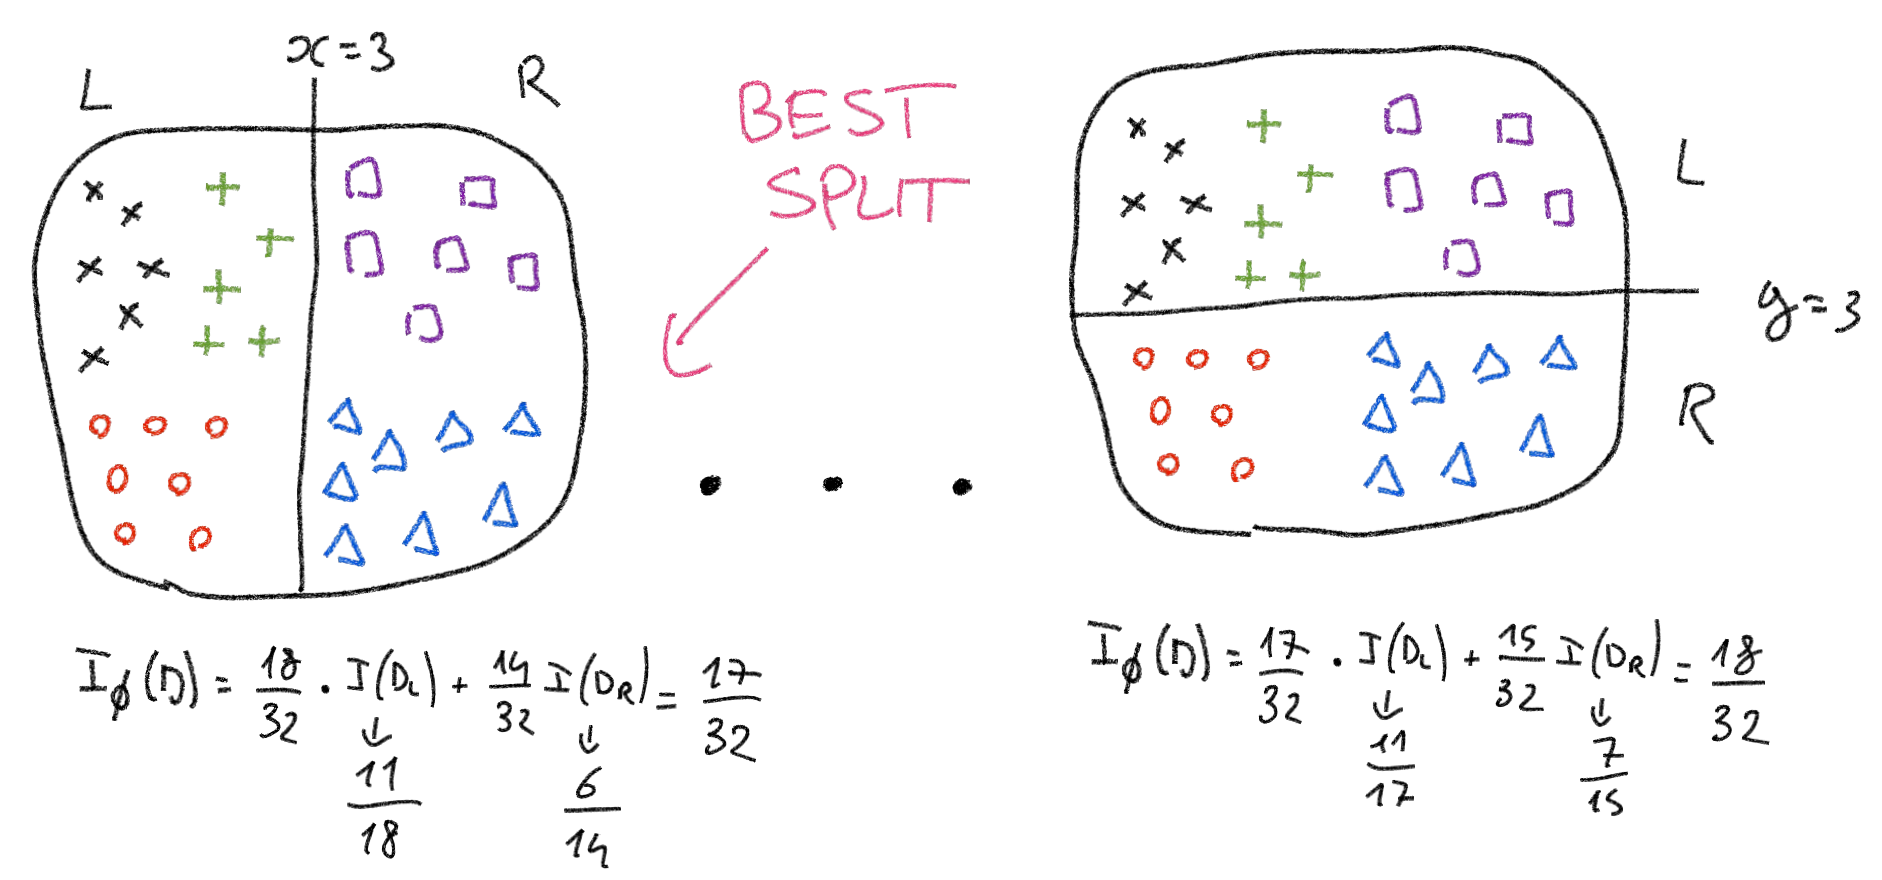
\includegraphics[scale=0.2]{split}

\section{Overfitting}
Because of the fact that they're determined by data, DT are particularly susceptible to overfitting. The usual techniques (regularization etc.) can be employed to avoid this, but there's also another called pruning.\\
This consists of taking a subtree and making it into a single node. This is usually done with subtress that are comprised of noisy data. \\
A {\bf random forest} is a collection of decision trees 
\chapter{Introduction to Neural Networks}
\begin{definition}[Artificial neuron]
	An artificial neuron (i.e. a perceptron) is a non linear parametrized function with restricted output range
\end{definition}

One example of perceptron is Rosemblatt (1958).

One problem with traditional perceptron is that it cannot solve the XOR: 
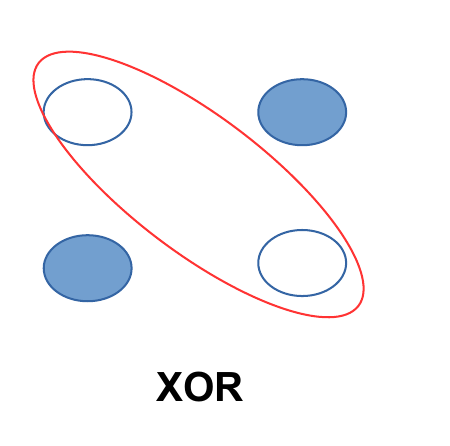
\includegraphics[scale=0.2]{xor}

because it is not linearly separable.

An idea to solve this is an {\bf MLP} (Multi Layered Perceptron), where the layers in between are intermediate results.

The problem now though is how to train an MLP. For perceptron we need to know the desired target and for hidden layers that is not the case. There are some ideas as follow. 
\newpage
{\bf Backpropagation}  was an idea to solve this problem, basically backpropagating the estimated error and updating the perceptron weights accordingly. \\
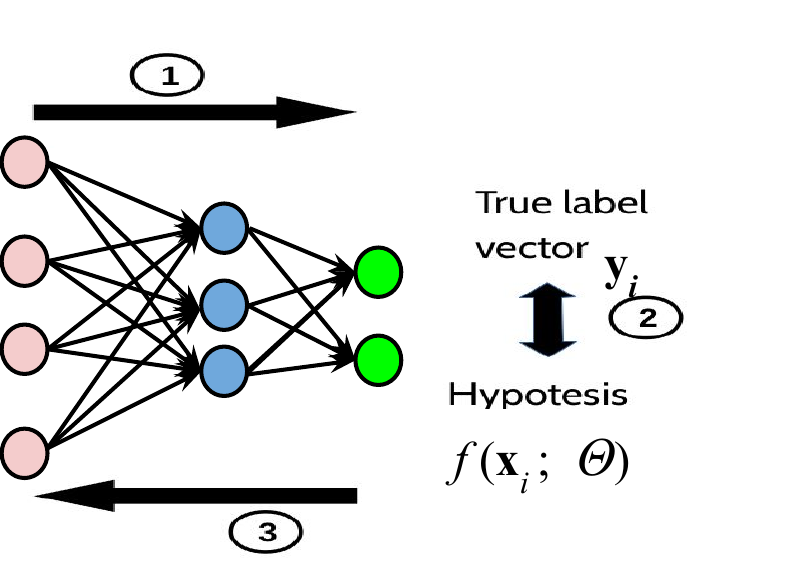
\includegraphics[scale=0.2]{backpropagation}

Now the problem was linked to the fact that neural networks cannot exploit many layers due to lack of computational power and overfitting. \\
Now neural networks reign supreme because of new findings. Raw data is always better than features and studies show that error rate is at an all time low. 

\begin{definition}[Neural Network]
	It's a composition of modules and a series of hierarchically connected functions, each with its own parameters.
\end{definition}

\section{Feedforward networks: basic elements}

The goal of a feedforward network is to approximate an idea function $f$. Information flows throughout the intermediate layers (hidden) to end on the last layer which is called output layer. \\
The function $f$ is a composite of the functions that comprise all the layers.\\
The {\bf training} is no different from other ML algorithms. \\
There are several modeling choices to be made:\\
{\bf COST FUNCTION}: for example cross-entropy or square loss\\
{\bf OUTPUT UNITS}: it's preferable to output probabilities (softmax) rather than linear outputs which could generate difficult gradient descent attributes. \\
The hidden unit accepts the input x and produces the output $h(z)$. The choice of $h$ (called {\bf ACTIVATION FUNCTION}) varies greatly. \\
{\bf ARCHITECTURE}\\
{\bf OPTIMIZATION }(see later)
\section{Backpropagation}
There are three steps to this:
\begin{enumerate}
	\item Feedforward propagation
	\item Use the computed output to calculate a scalar cost depending on the loss function
	\item Backpropagation
\end{enumerate}

The main idea of backpropagation is to use gradient descent. We do not know how or which of the hidden units are wrong but we can infer with gradient descent the speed at which we're getting farther from the correct output.


\chapter{Optimization for Neural Networks and CNNs}
The optimization of a NN comes with more learning. \\
The main idea is to adjust all the weights of the network $\theta$ such that the cost function is minimized. Formally:\\
\[
min_\theta \sum_i L(y_i, f(x_i, \theta))
\]

To do this, usually we use gradient descent and back propagation, although there are different methods. 
\section{Batch (Stochastic) Gradient Descent (BGD) and (SGD) }
The main idea is that the learning rate $\eta$ changes linearly. \\
The update to the weights (w) is: \\
$w = w - \eta_k g$

Pros: estimates are stable \\
Cons: needs to estimate the GD throughout the whole training.

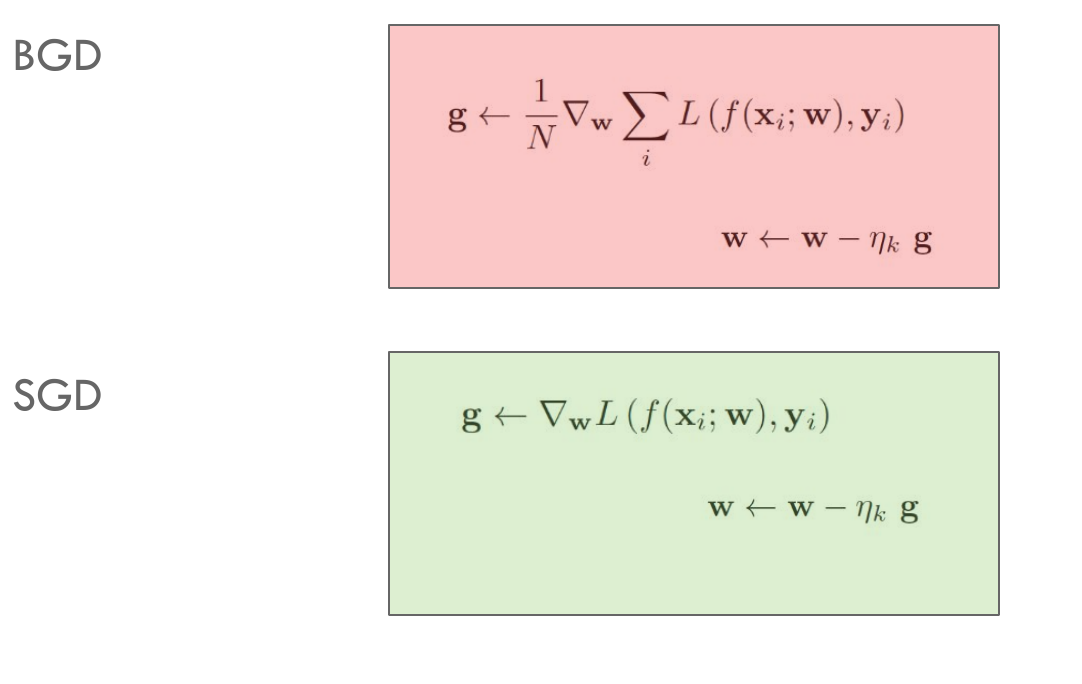
\includegraphics[scale=0.18]{bdg}

Gradient descent estimates can be very noisy so a solution is to reduce the number of batches (minibatches).\\
Another problem has to do with momentum: SGD can be very slow, so we introduce a new variable: velocity ($v$)

\section{Convolutional Neural Networks (CNNs)}
Neural networks are particularly effective when the data is spatial (i.e. language and images).

For images for instance each layer extract features from the previous output. 
\begin{definition}[Convolutional Neural Networks]
	A CNN is a neural network in which it uses convolution in at least one of its layers
\end{definition}
Okay, cool, but what is convolution? \\
Convolution is a general purpose filter operation for images. A kernel matrix is applied to images and it works by determining the central value of a pixel and adding the weights of all its neighbors.\\
In CNN's architecture there are 3 main operations:
\begin{itemize}
	\item Convolution
	\item Non-linearity
	\item Pooling
\end{itemize}

Convolution consist of learned filters. The idea is that each filter is supposed to give insight on a specific type of feature. \\
Pooling consists of reducing the spatial size of the representation: this reduces the number of parameters and controls overfitting.\\
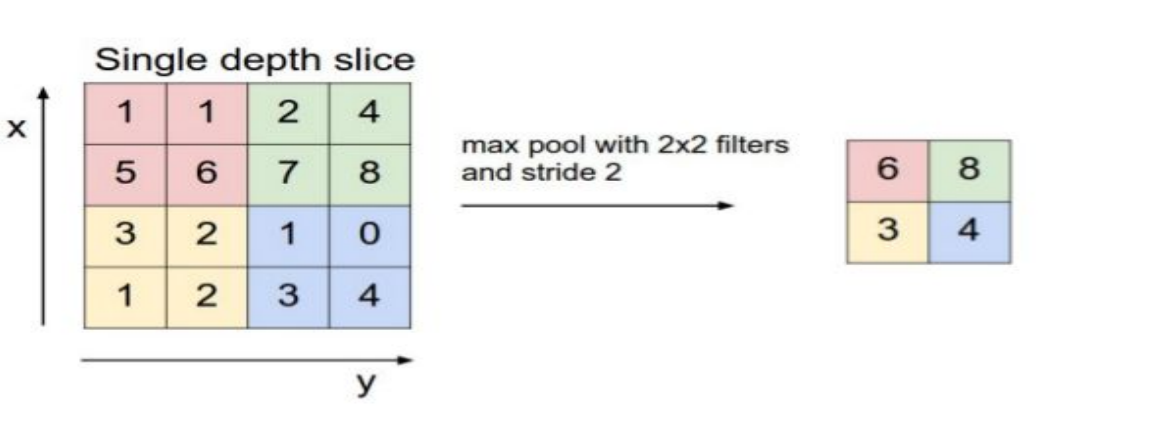
\includegraphics[scale=0.4]{pooling}

\chapter{Unsupervised Learning}
whiUnsupervised learning works by observing data distribution ${\bf P}_data$,  while lacking a target variable.\\
There are several applications to this: \\
{\bf DIMENSIONALITY REDUCTION}, find a function f that maps each input $x \in \mathscr{X}$ to a lower dimensional embedding, where dim($\mathscr{Y}$) $ < $ dim($\mathscr{X}$). \\
Why would one want to do this? By compressing the input data we also reduce the feature dimensionality making the input more lightweight thus reducing the time for data elaboration.\\
{\bf CLUSTERING} finds a function $f$ that assigns each input $x \in \mathscr{X}$ to a cluster. Why? \\
It allows to analyze data by grouping it together and can also be used to compress data with similar patterns.\\
{\bf DENSITY ESTIMATION} find a probability distribution $f \in \triangle \mathscr{X}$ that fits the data $x \in \mathscr{X}$. Why? 
Allows for explicit estimate of an unknown probability distribution, generating new data and detecting anomalies.\\
\section{Principal component analysis}
The main idea is to fidn the direction of maximum variance, change the coordinate system and then dropping dimensions of least variance. \\
\begin{definition}[Variance and Covariance]
	Measure of the spread of a set of points around their center of mass (the mean)
\end{definition}

I don't really know how to explain easily eigenvalues and eigenvectors so I'm just gonna put a picture of the example.
\\
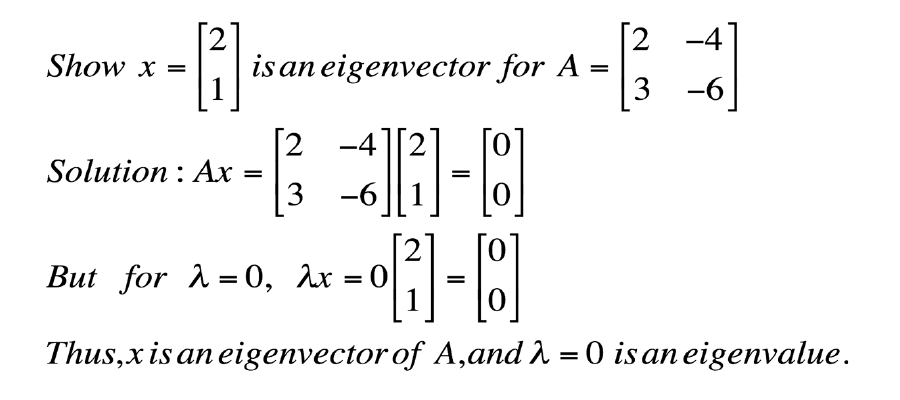
\includegraphics[scale=0.5]{eigen}

It can be shown that the largest eigenvalue is the variance along the first principal component.

\section{Clustering}
The goal is to divide data into clusters. What K-means clustering does is fix a number of k clusters and divides the data with the least amount of variance inside the clusters.
\[
min \sum_{j=1}^{k}V(\mathscr{C})
\]
Some properties are that it is sensitive to the scale of features, it is guaranteed to converge although it's not guaranteed to find a global minimum. \\
The problem with K-means clustering is that it requires spherical clusters. It is also a {\bf hard cluster}, meaning that example belong exactly to one cluster only. \\
{\bf EM-Clustering } (Expectations Maximization) on the other hand is a soft clustering technique that takes data as a mixture of gaussian.

With EM clustering you start with initial cluster centers, you soft assign points to each cluster and then iterate.\\
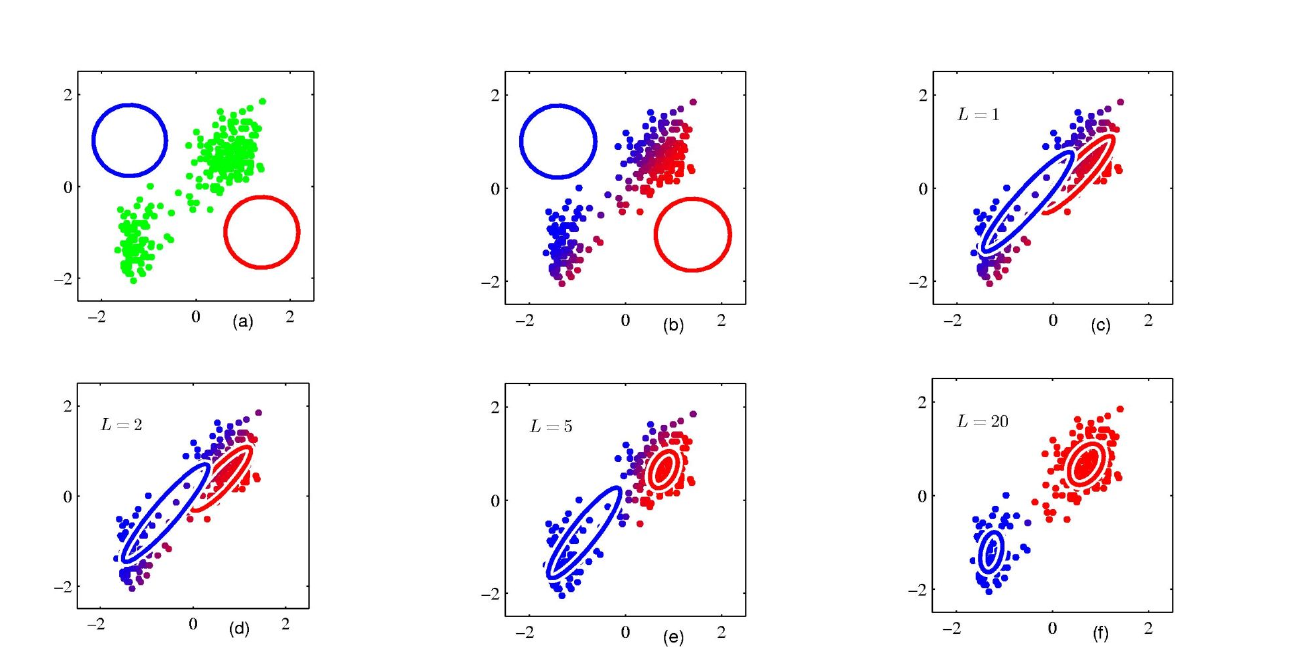
\includegraphics[scale=0.3]{em}
To recalculate the centers we need them to fit a gaussian.

There are other means of clustering namely spectral clustering (using graphs), hierarchical graphs, agglomerative clustering etc.
\end{document}